\documentclass{article}

% if you need to pass options to natbib, use, e.g.:
%     \PassOptionsToPackage{numbers, compress}{natbib}
% before loading neurips_2018

% ready for submission
% \usepackage{neurips_2018}

% to compile a preprint version, e.g., for submission to arXiv, add add the
% [preprint] option:
%     \usepackage[preprint]{neurips_2018}

% to compile a camera-ready version, add the [final] option, e.g.:
%	  \usepackage[final]{neurips_2018}

% to avoid loading the natbib package, add option nonatbib:
%     \usepackage[nonatbib]{neurips_2018}

\usepackage[utf8]{inputenc} % allow utf-8 input
\usepackage[T1]{fontenc}    % use 8-bit T1 fonts
\usepackage{hyperref}       % hyperlinks
\usepackage{url}            % simple URL typesetting
\usepackage{booktabs}       % professional-quality tables
\usepackage{amsfonts}       % blackboard math symbols
\usepackage{nicefrac}       % compact symbols for 1/2, etc.
\usepackage{microtype}      % microtypography
\usepackage{graphicx}  % inclusion of graphics; see: http://en.wikibooks.org/wiki/LaTeX/Importing_Graphics
% allow easy inclusion of .tif, .png graphics

\DeclareGraphicsRule{.tif}{png}{.png}{`convert #1 `dirname #1`/`basename #1 .tif`.png}
\usepackage{float}
\usepackage{subfigure}  % allows subfigures in figure


\title{Generating and Analyzing Handwritten Devanagari Digits using Generative Adversarial Network}

% The \author macro works with any number of authors. There are two commands
% used to separate the names and addresses of multiple authors: \And and \AND.
%
% Using \And between authors leaves it to LaTeX to determine where to break the
% lines. Using \AND forces a line break at that point. So, if LaTeX puts 3 of 4
% authors names on the first line, and the last on the second line, try using
% \AND instead of \And before the third author name.

\author{%
  Lien, I-Chun \\
  Department of Electrical and Computer Engineering\\
  University of Arizona\\
  \texttt{ichunlien@email.arizona.edu} 
  \\[3ex]
  Gupta,  Srishti  \\
  Department of Electrical and Computer Engineering\\
  University of Arizona\\
  \texttt{srishtigupta1@emial.arizona.edu} 
%
}

\begin{document}
% \nipsfinalcopy is no longer used

\maketitle

\begin{abstract}
  In this project, we’re going to generate handwritten Devanagari numerals. The generative adversarial network(GAN) can generate the synthetic data by training discriminator and generator. The discriminative model is to determine the likelihood of the real and generated handwritten Devanagari numerals. The generative model is to generate the fake data for fooling the discriminative model. Both of the models can improve over epochs. The propose of the training process is to train a generator to create handwritten numerals. We observed and analyzed the performance of the generator by adjusting activation function and regularizer.
\end{abstract}

\section{Introduction}

\paragraph{}
Generative adversarial network, an application of machine learning, is useful for realistic data-limit situation. Because collecting real data is difficult and time-consuming in most of the case, we can use GAN to generate new data from training data. GAN is using discriminative model to update generative model for fooling machines to determine whether the images are fake or real. There are 20000 sets of  Hindi digit in the dataset. We want more training images for digit recognition, so using GAN to generate synthetic data proposed as a form of generator for semi-supervised learning. 
Following are the steps GAN take:
i)	Generator takes a fixed-length random vector as input and returns some image from the domain.
ii)	The generated image is fed in discriminator along with a stream of actual ground-truth images 
iii)	The discriminator takes in both real and fake images and returns probabilities 0 or 1, where 0 represents fake and 1 represents authenticity.
iv)	Analysis of GAN output while changing hyperparameters of the model is done.
\paragraph{}
The parameter of the convolutional network, regularization function, and activation function all affect the GAN model. However, there are some problems in generative adversarial network like non-convergence, mode collapse, sensitive for the parameter selection. 




\section{Background}
\paragraph{}
Devanagari is an Indic script that forms a basis of over 100 languages spoken in India, Nepal and Bangladesh including Hindi, Maithili, Sanskrit etc. It consists of 47 essential alphabets 10 digits. Hindi is most spoken language in India and is third most popular language in the world. Other than Hindi, other languages such as Marathi, Maithili, Sanskrit etc. are coded in Devanagari. Basic digits in Devanagiri consists of 10 numbers [1] as shown in Fig. 1.
\begin{figure}[ht]
	\centering
	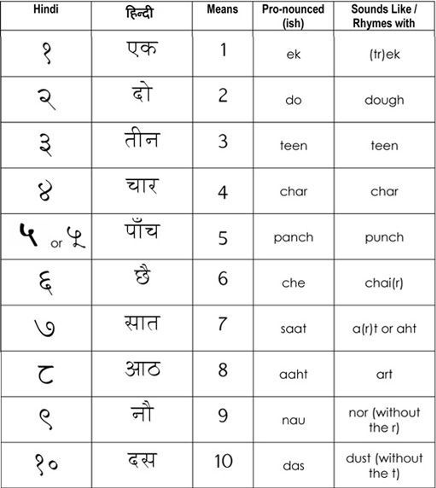
\includegraphics[width=8cm]{figs/Picture1}
	\caption{Devanagari Digits.}
\end{figure}
\paragraph{}
Character Recognition is the identification of printed characters from an image, a handwritten note, books, letters, and cheques. However, recognizing handwritten digit is a challenging problem not only in the field of Optical Character Recognition (OCR) but also in the perspective of behavioral biometrics. Writing is the most natural mode of storing and transmitting information. The research effort [2] in the field of OCR was due to challenges on simulation of human reading and also because of its potential applications, for example, in postal automation, bank cheque analysis and processing, conversion of handwritten text into Braille, hand drawn pictogram or formula recognition, and so forth. One of the major reasons for the absence of sustained research effort in Devanagari OCR is the deficiency o the data resources. Ground-truthed data for words and characters, on-line dictionaries, corpora of text documents, reliable standardized statistical analysis, and evaluation tools are currently lacking. So, the creation of data resources will undoubtedly provide a much-needed fillip to researchers working on Devanagari OCR.
\paragraph{}
Generative Adversarial Network, or GAN is an approach to generative modeling, which is an unsupervised learning task in machine learning. GAN is a clever way of training a generative model by framing the problem as supervised model with two sub-models: the generator that generates new data instances, whereas, the discriminator evaluates them for authenticity by classifying the as either real (form domain) or fake (from generator). The two sub-models [3] are trained together in a zero-sum game adversarial, until the discriminator model is fooled about half the time, meaning the generator model is generating plausible examples. The objective function is given by:
\begin{figure}[ht]
	\centering
	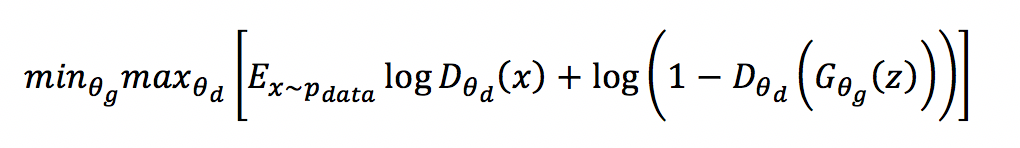
\includegraphics[width=7cm]{figs/eq1}
\end{figure}

\paragraph{}
Where \( D_{\theta_d}(x)\)  is the discriminator output of real data \(x\) and \(D_{\theta_d} (G_{\theta_g}(z))  \)s the discriminator output for generated fake data \(G(z)\). The objective function represents a minimax function as discriminator tries to maximize the objective function and hence perform gradient ascent on objective function, whereas, generator tries to minimize the objective function and therefore performs gradient descent function. 

\paragraph{}
Following is a GAN model with hidden layers used in this project.

\begin{figure}[H]
	\centering
	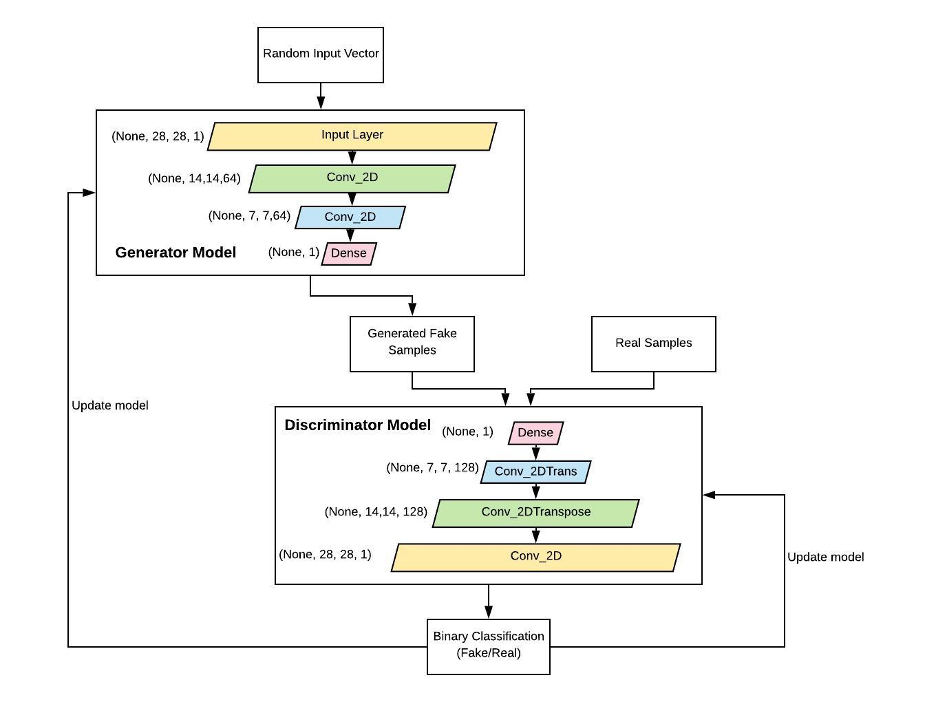
\includegraphics[width=10cm]{figs/Picture2}
	\caption{Gan model used in the project.}
\end{figure}

\paragraph{Generator Model}
From the name it suggests, generator model is used to generate images in the domain by taking fixed-length random vector as input. This vector is used to seed the generative process. After training, points in this multidimensional vector space, which we call the latent variables, corresponds to points in the problem domain, forming a compressed representation of the data distribution. The generator model applies meaning to points in a chosen latent space, such that new points drawn from the latent space can be provided to the generator model as input and used to generate new and different output examples. In this project, function “latentpoints” is doing this job. Fig. 3 is a snippet from the code performing the function.
\begin{figure}[H]
	\centering
	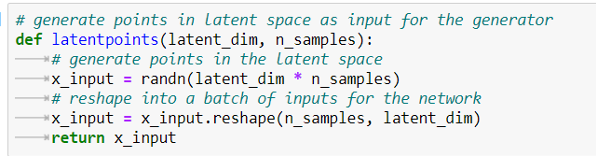
\includegraphics[width=10cm]{figs/Picture3}
	\caption{Latent dimensionality function used in the code.}
\end{figure}

\paragraph{Discriminator  Model}
Discriminator model is a normal classification model which takes real input from the training dataset and fake input from generator model and discriminate fake from real. After training, discriminator model is discarded as our interest lies in generated samples.

\paragraph{Issues with GAN}
Since GAN is double feedback loop, it may suffer from following [4] problems: 

\begin{itemize}
	\item Mode Collapse: the generator produces limited variety of samples as it collapse while training.
	\item Non-Convergence: model parameters oscillate, destabilize, and never converges.
	\item Diminished gradient: generator gradient vanishes as discriminator gets too successful and learns nothing eventually.
	\item Sensitivity: model becomes highly sensitive to hyperparameters.
	\item Overfitting: imbalance between generator and discriminator leads to overfitting.
\end{itemize}

Possible reason behind non-convergence: \textbf{Nash Equilibrium}.
GAN is based on non-zero non-cooperative game, also called minimax. The opponent wants to maximize its action and minimize your action. According to game theory, GAN model reaches convergence when both generator and discriminator model reaches Nash Equilibrium [4], which is the optimal point of the objective function: 

\begin{figure}[H]
	\centering
	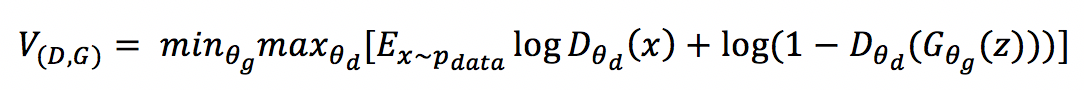
\includegraphics[width=10cm]{figs/eq2}
\end{figure}

Since both sides want to undermine the others, a Nash equilibrium happens when one player will not change its action regardless of what the opponent may do. In other words, because the opponent always countermeasures other’s action that makes the model harder to converge.

\section{Results and analysis}
\label{headings}

\paragraph{}
Although, generally, there is no objective way to evaluate the performance of GAN model. It is very difficult to calculate objective error score for generated images, instead, subjective evaluation is the best tool so far. This is done by a human observer and hence, we will not know when to stop training without looking at samples of generated images. For serving the purpose, we ran our model for different activation functions, regularizers and different kernel values of convolutional 2D layers and analyzed the performance using fake and real accuracy on discriminator and loss on discriminator and generator, as performance metrics. In this paper, we present, few of our observations:

\subsection{Parameter Set-1}
\begin{itemize}
	\item Output layer regularizer: \textbf{Dropout (p = 0.4)}
	\item Discriminator activation function:  \textbf{sigmoid}
	\item Generator activation function:  \textbf{sigmoid}
\end{itemize}

\begin{figure}[H]
	\centering
	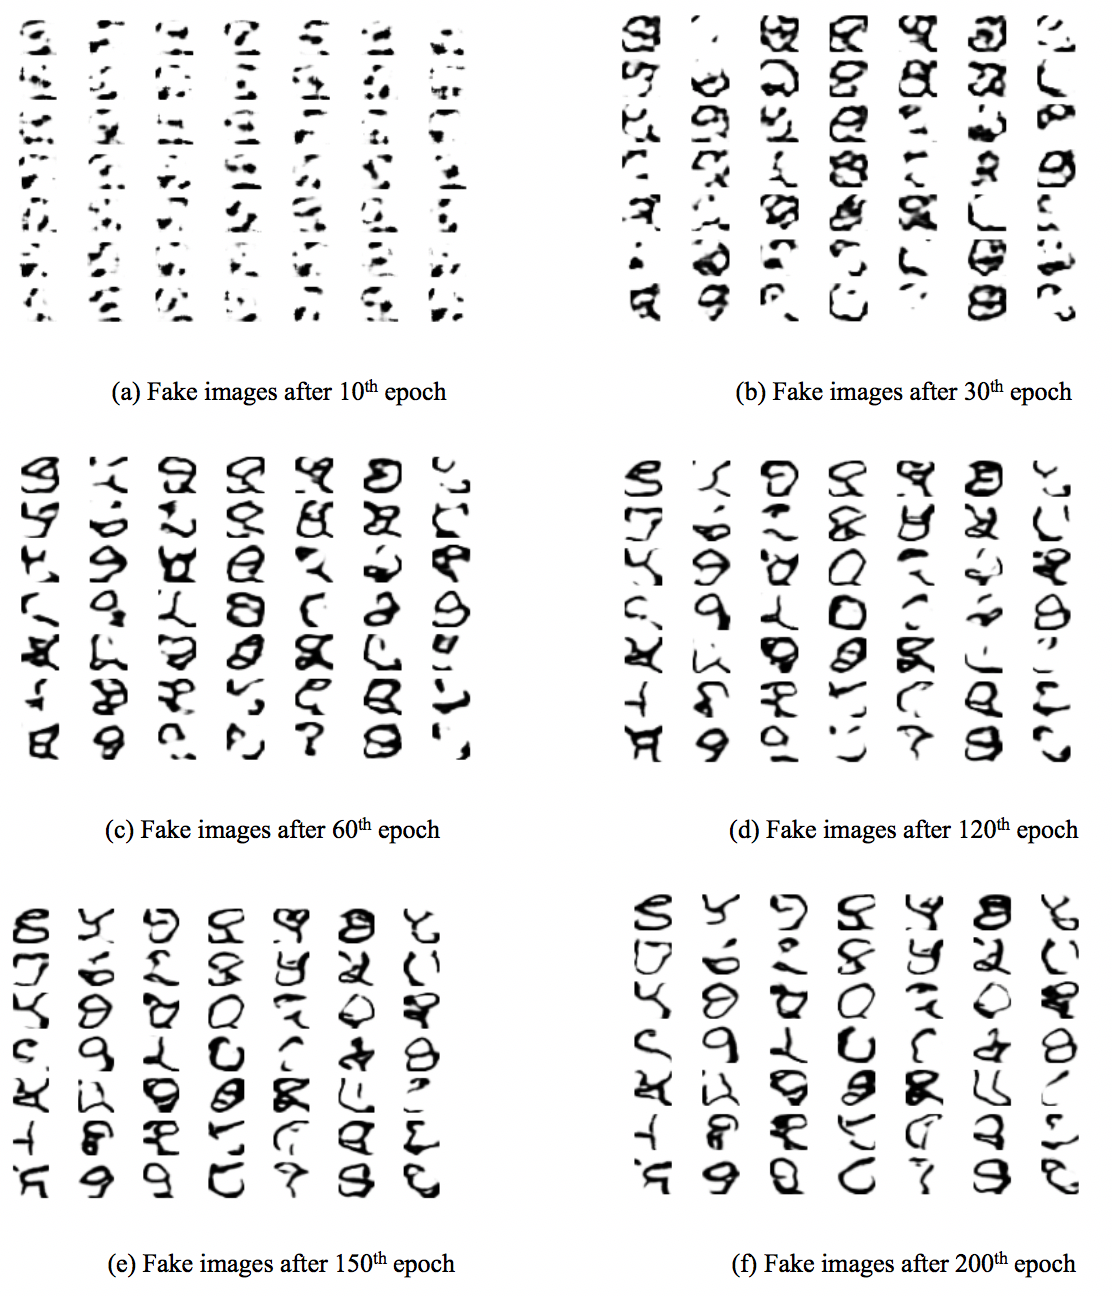
\includegraphics[width=10cm]{figs/Picture4}
	\caption{Fake images with dropout=0.4 after 10, 30, 60, 120, 150, 00 epoch.}
\end{figure}

\paragraph{}
On using GAN model with sigmoid activation function in generator as well as discriminator and using dropout with probability of retention as 0.4 in discriminator, we observed that after first 10 epochs, we get noisy gibberish values, however, images begins to get in shape by 30-40th epoch, we seem some reasonable images in 60th epoch. After 60-70th epoch, we observe the images tend to remain more or less similar with slight change in blocky-ness of images. We also observe that after 70th epoch, digit samples tend to oscillates in their weights and not necessarily improvising it from before. 
Following graph compares the error on discriminator model and generator model based on discriminator’s error.

\begin{figure}[H]
	\centering
	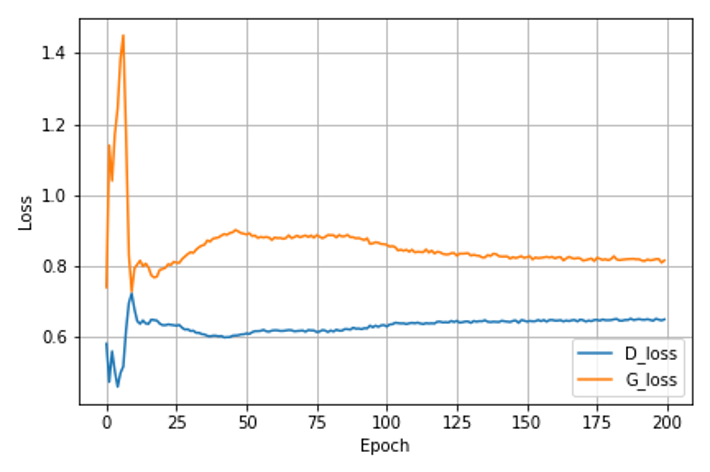
\includegraphics[width=7.5cm]{figs/Picture5}
	\caption{Loss graph for activation function in D as sigmoid ,G as sigmoid, Dropout = 0.4.}
\end{figure}

From the plot below, we observe that losses in both the models tend to converge close to 100 epochs with error rate of 0.85 in generator and 0.65 in discriminator.

\subsection{Parameter Set-2}
\begin{itemize}
	\item Output layer regularizer: \textbf{Dropout (p = 0.2)}
	\item Discriminator activation function:  \textbf{sigmoid}
	\item Generator activation function:  \textbf{sigmoid}
\end{itemize}


\begin{figure}[H]
	\centering
	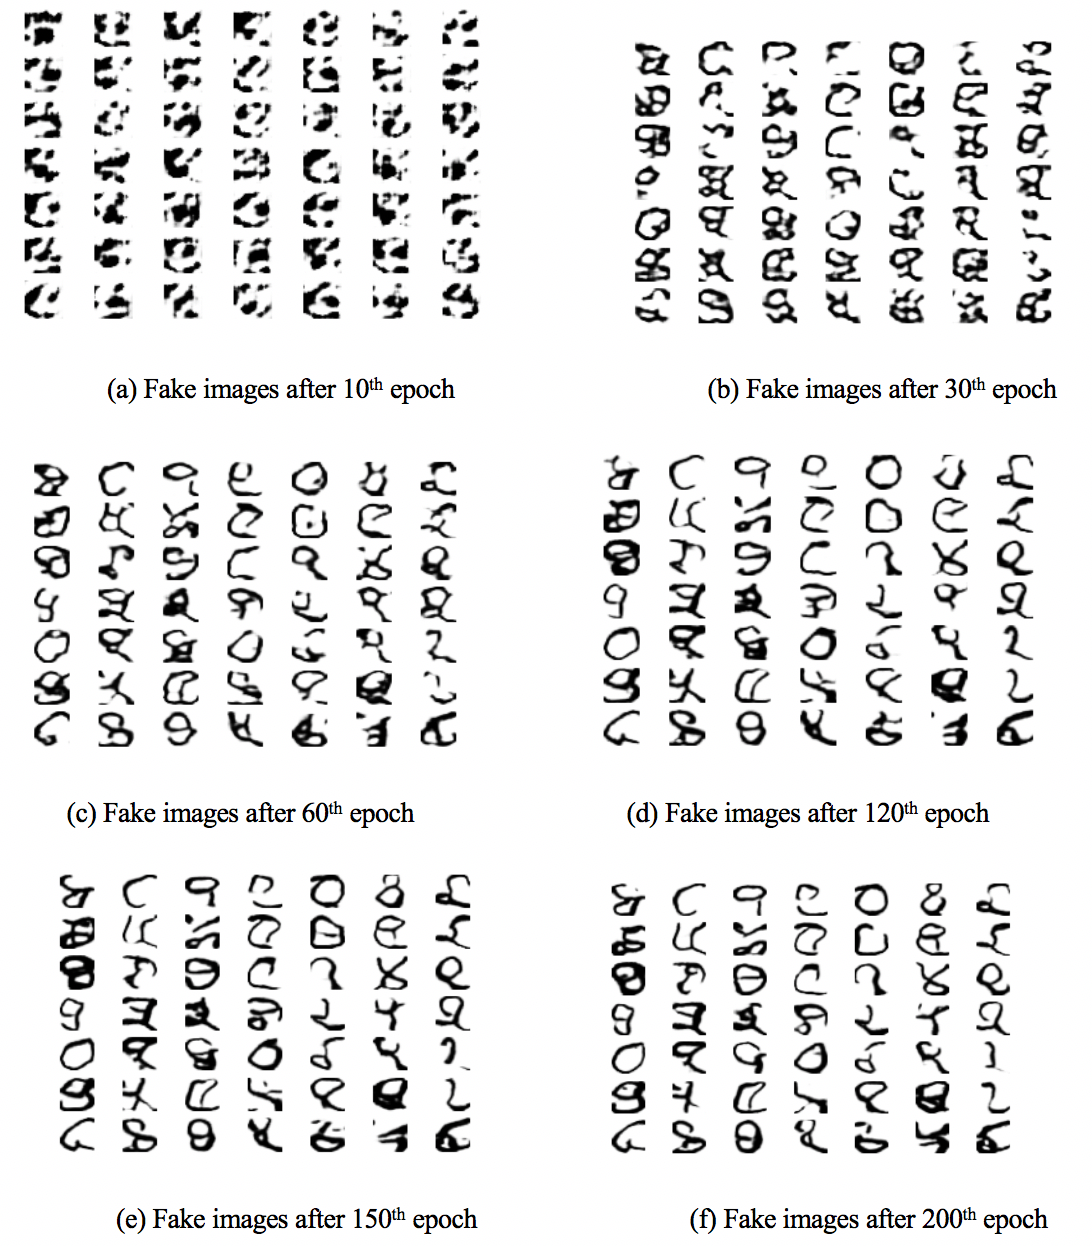
\includegraphics[width=10cm]{figs/Picture6}
	\caption{Fake images with dropout=0.2 after 10, 30, 60, 120, 150, 00 epoch.}
\end{figure}

\paragraph{}
On using GAN model with sigmoid activation function in generator as well as discriminator and using dropout with probability of retention as 0.2 in discriminator we notice the gibberish data at or around10th  epoch, which does not resemble the original digits at all. Whereas, at the end of 40th epoch, we do see some formation in digits, for example, image[7,1] is an English 8, image[3,6] is an English 4. We also observe that images do not change drastically in further epochs. 
\paragraph{}
Graph in Fig. 7 substantiates the above obeservations as both the errors tend to converge at 40th epoch getting both the values close to 0.7. Here, we also notice that generator error falls from 0.85 in same model having dropout 0.4 to 0.7 in model having dropout with probability 0.2.


\begin{figure}[H]
	\centering
	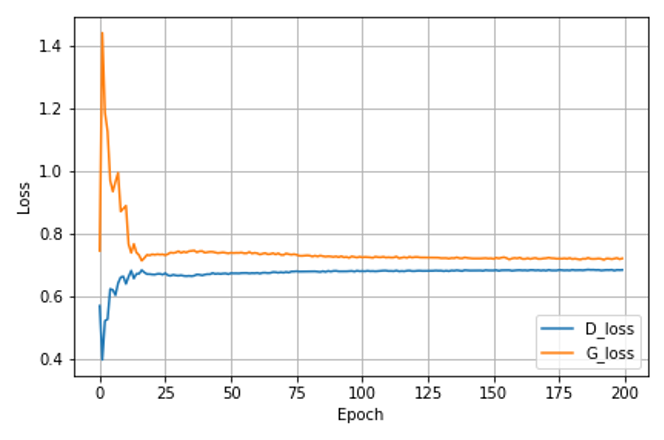
\includegraphics[width=7.5cm]{figs/Picture7}
	\caption{Loss graph for activation function in D as sigmoid ,G as sigmoid, Dropout = 0.2.}
\end{figure}



\subsection{Parameter Set-3}
\begin{itemize}
	\item Output layer regularizer: \textbf{Dropout (p = 0.2)}
	\item Discriminator activation function:  \textbf{tanh}
	\item Generator activation function:  \textbf{sigmoid}
\end{itemize}

\begin{figure}[H]
	\centering
	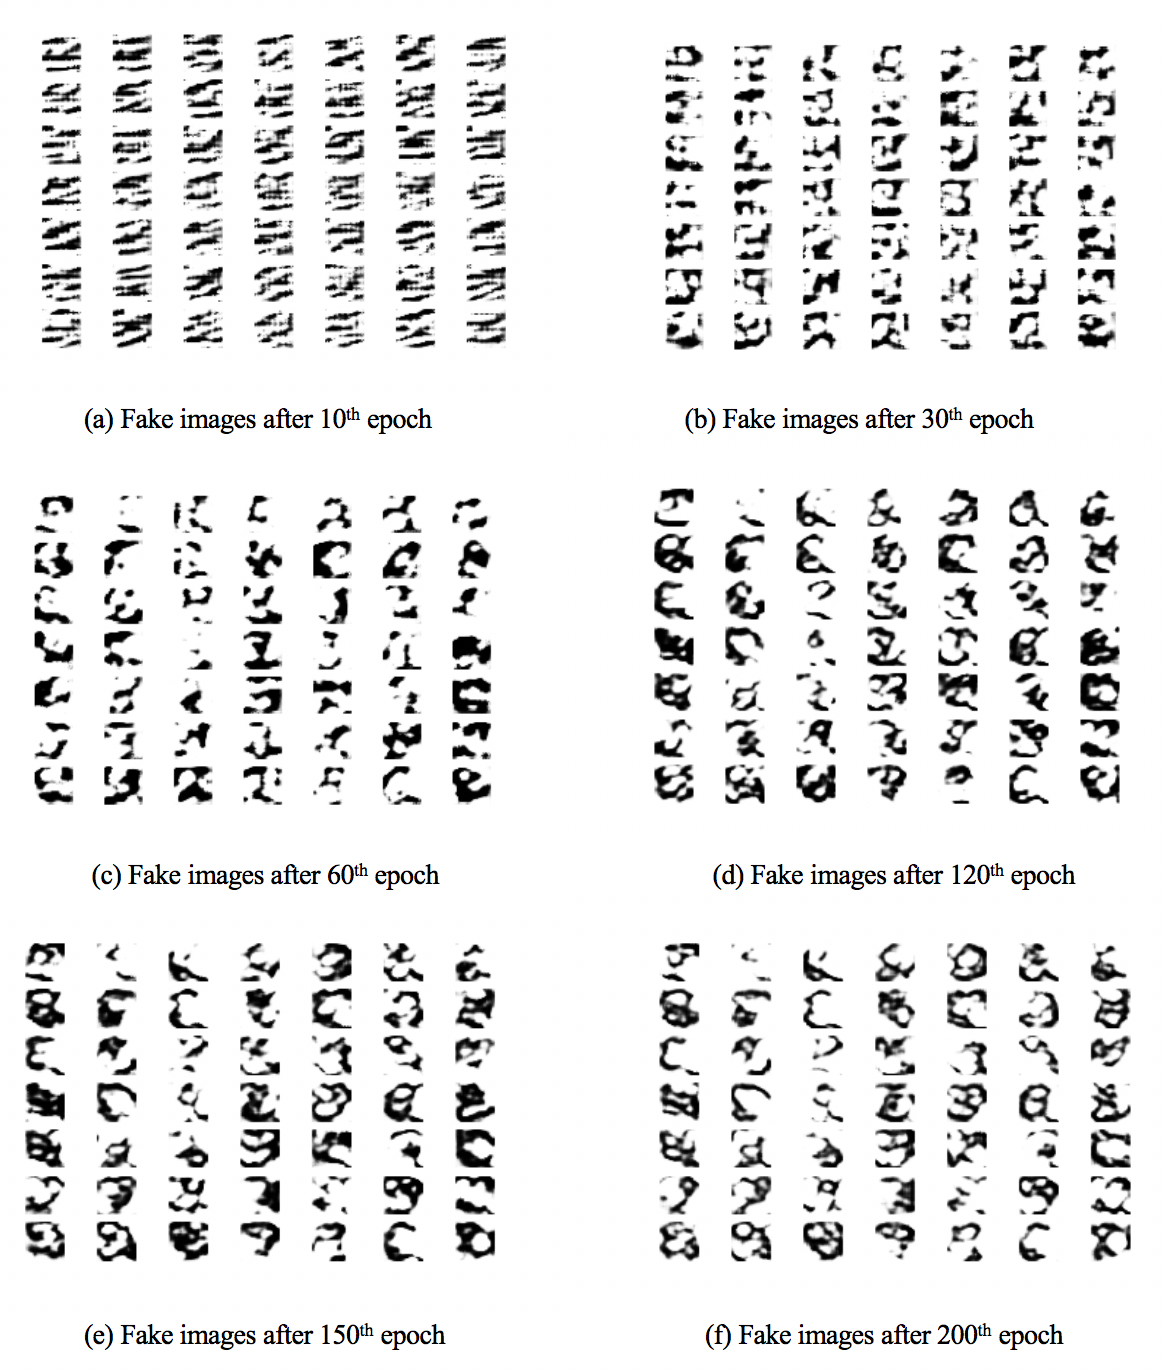
\includegraphics[width=10cm]{figs/Picture8}
	\caption{Fake images with discriminator activation function: tanh/ generator activation function: sigmoid.}
\end{figure}

\paragraph{}
On using GAN model with tanh activation function in generator and sigmoid in discriminator and using dropout with probability of retention as 0.2 in discriminator, we  againobserved that after first 10 epochs, we get noisy gibberish values. However, in this case images do not tend to improve, rather it stays gibberish even till 200th epoch. Although, we notice change in weights, but useful information is not observed.
\paragraph{}
In the following plot in Fig 9, we observe that loss in generator model doesn’t converge at all, atleast not until 200 epochs. It is likely, that it might converge close to 300 epochs. Although it is cleas that $d_loss$ has constant low values close to 0.5 with peaks at certain places. Due to such small values of discriminator model, it can also be said that generator is not performing well enough to fool the discriminator.


\begin{figure}[H]
	\centering
	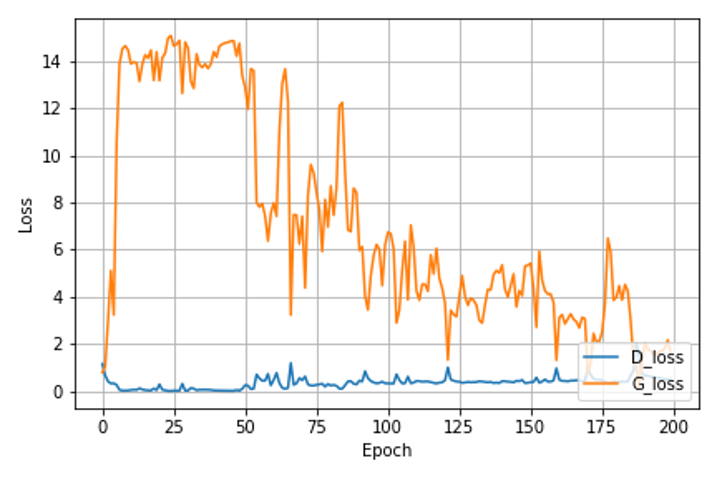
\includegraphics[width=7.5cm]{figs/Picture9}
	\caption{Loss graph for activation function in D as tanh ,G as sigmoid, Dropout = 0.2.}
\end{figure}


\subsection{Parameter Set-4}
\begin{itemize}
	\item Output layer regularizer: \textbf{Dropout (p = 0.2)}
	\item Discriminator activation function:  \textbf{sigmoid}
	\item Generator activation function:  \textbf{ReLU}
\end{itemize}

\begin{figure}[H]
	\centering
	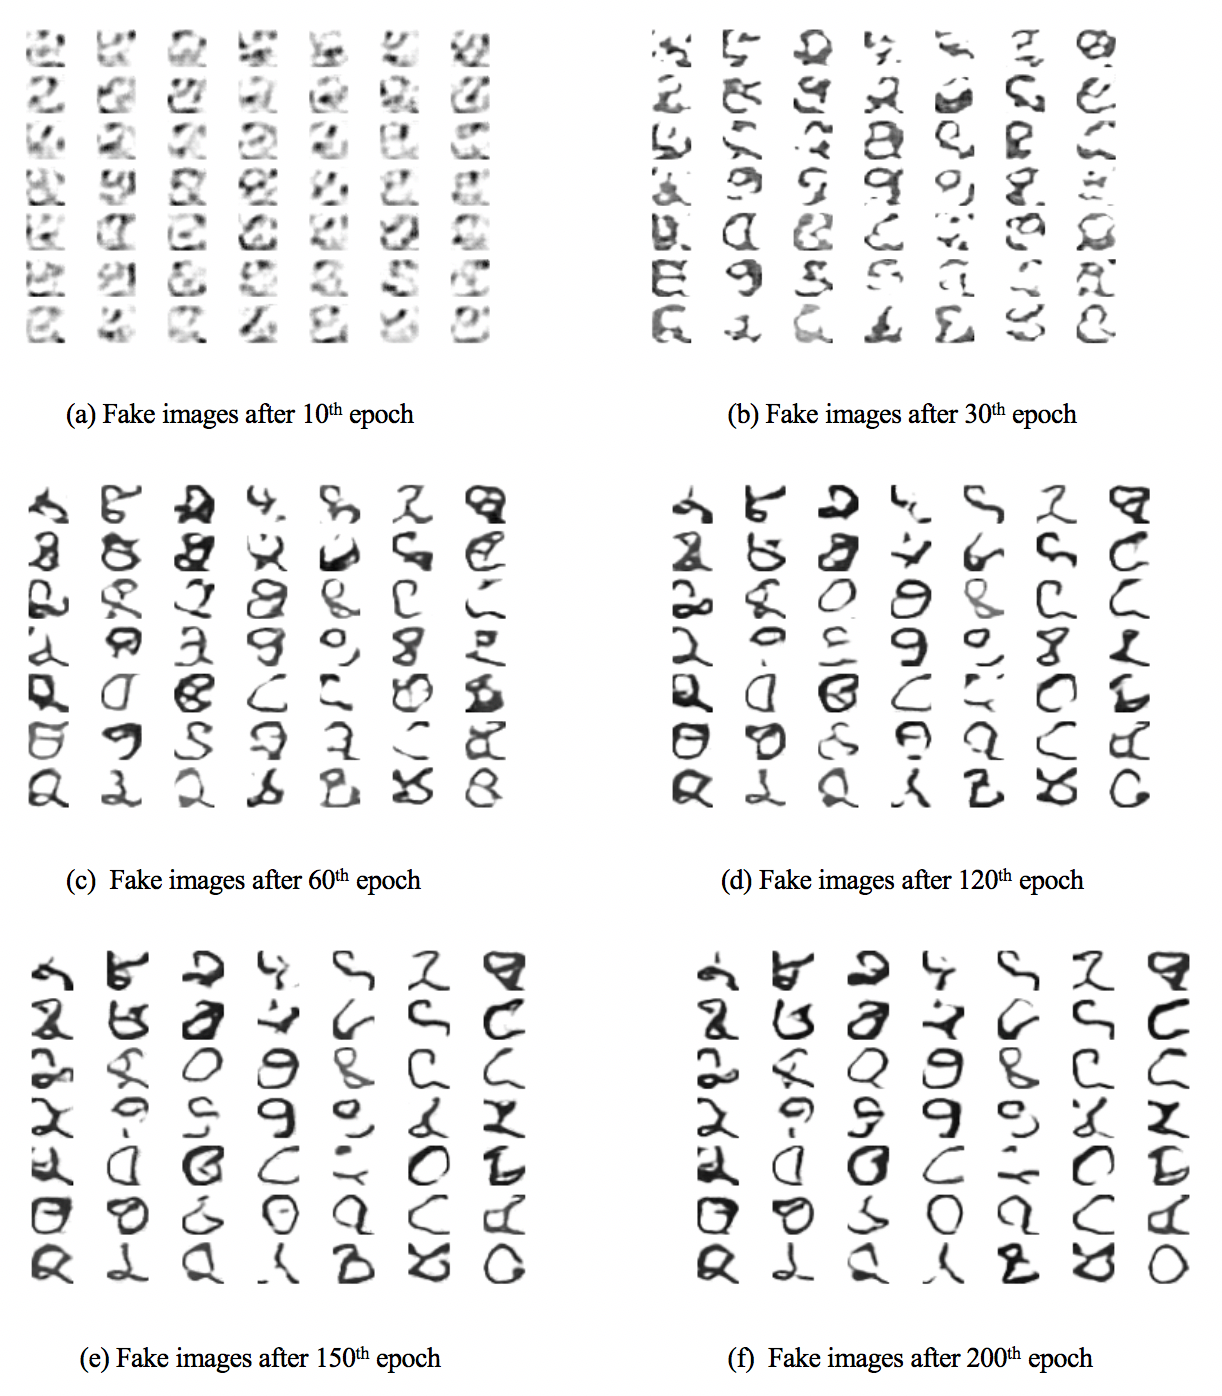
\includegraphics[width=10cm]{figs/Picture10}
	\caption{Fake images with discriminator activation function: sigmoid/ generator activation function: ReLU.}
\end{figure}

\paragraph{}
On using GAN model with sigmoid activation function in generator as well as discriminator and using dropout with probability Following figures Fig. 10, shows the output of the GAN model with sigmoid as activation function in discriminator and ReLU in generator having dropout with probability of retention as 0.2 in discriminator. We observe the regular trend of getting gibberish images in first 10-20 epochs. Although, it does not show meaningful data until 60-70th epoch. From Fig. 10, we can observe good images, for example, image[4,1] is and English 2, image[7,6] is an English 4, image[7,7] is an English 8. Images do not tend to improve approximately after 100 epochs. We also observe that after 80th epoch, digit samples tend to oscillates in their weights and not necessarily improvising it from before.


\begin{figure}[H]
	\centering
	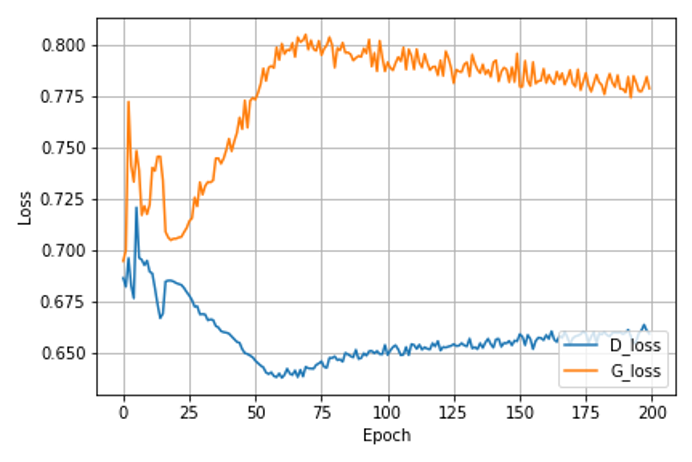
\includegraphics[width=7.5cm]{figs/Picture11}
	\caption{Delineates the losses by both the sub-models. We observe that both $d_loss$ and $g_loss$ start converging at 70 epochs with loss of $0.65$ and $0.8$ declining a bit to $0.78$ at close to $120$ epochs.}
\end{figure}




\section{Conclusion}
\label{others}

After analyzing all the outputs, we observe that change in hyperparameter very much affects the GAN output. Also, we noticed, it performed relatively better on using optimizer Dropout with probability of retention 0.2 in discriminator and activation function at Generator as sigmoid and for discriminator as sigmoid as well. Also, we observe that $d_loss$ and $g_loss$ tends to converge after certain epochs, without improvising the digits much. Please find the code on Github 
\begin{center}
	\url{https://github.com/srish01/ML-Project}
\end{center}


\section*{References}



\medskip
\small

[1] Google images https://in.pinterest.com/pin/515521488568785608/

[2] P. Singh, A. Verma, N.S. Chaudhari, “On the Performance Improvement of Devanagari Handwritten Character Recognition”, Applied Computational Intelligence and Soft Computing, 2015 

[3] J. Brownlee, “A Gentle Introduction to Generative Adversarial Networks (GANs)”. 2019

[4] Jonathan Hui, “GAN — Why it is so hard to train Generative Adversarial Networks!”, Medium Data Science

[5] Goodfellow, Ian, et al. "Generative adversarial nets." Advances in neural information processing systems. 2014.

[6] Mescheder, L., Geiger, A., Nowozin, S. (2018). Which training methods for GANs do actually converge?. arXiv preprint arXiv:1801.04406.

[7] Goodfellow, I. (2016). NIPS 2016 tutorial: Generative adversarial networks. arXiv preprint arXiv:1701.00160.

[8] Brownlee, J. (2019, October 3). How to Reduce Overfitting With Dropout Regularization in Keras. Retrieved from https://machinelearningmastery.com/how-to-reduce-overfitting-with-dropout-regularization-in-keras/

[9] Hui, J. (2020, March 10). GAN - Ways to improve GAN performance. Retrieved from https://towardsdatascience.com/gan-ways-to-improve-gan-performance-acf37f9f59b

[10] Znxlwm. (2017, August 9). znxlwm/tensorflow-MNIST-GAN-DCGAN. Retrieved from https://github.com/znxlwm/tensorflow-MNIST-GAN-DCGAN


\end{document}